\documentclass [a4paper] {report}
\usepackage{amsmath,amssymb,amsthm, bbm, graphicx,listings,braket,subfig,titlesec,cleveref,lipsum,mcode,xcolor-patch, textcomp,float,booktabs,siunitx, listings}
\usepackage[authoryear]{natbib}
\usepackage[section]{placeins}
\usepackage[margin=2.2cm]{geometry}
\titleformat{\chapter}{\normalfont\huge}{\thechapter.}{20pt}{\huge \bf}

\DeclareMathOperator*{\argmin}{arg\,min}
\DeclareMathOperator*{\argmax}{arg\,max}
\newcommand{\norm}[1]{\left\lVert #1 \right\rVert}

\begin{document}
	
	\begin{titlepage}
		\begin{center}
			
			\textsc{\LARGE IN4320 Machine Learning}\\[1.25cm]
			
			\rule{\linewidth}{0.5mm}\\[1.0cm]
			{\huge \bfseries Exercise Computational Learning Theory: Boosting }\\[0.6cm]
			\rule{\linewidth}{0.5mm}\\[1.5cm]
			
			\begin{minipage}{0.4\textwidth}
				\begin{flushleft} \large	
					\emph{Author:}\\
					\textsc{Milan Niestijl, 4311728}
				\end{flushleft}
			\end{minipage}
			
			\vfill
			{\large \today}
		\end{center}
	\end{titlepage}
	
	\section*{a.}
	Let $x\geq0$. then $e^{-x} \geq (1-x)$.\\
	\subsection*{Proof:}
	Note that $e^{-x} \geq 0$ and $e^{0} = 1$, so that the result is trivial for $x\geq 1$ and $x=0$. We assume $x \in (0,1)$. Then we have, using the Taylor series representation of $e^{-x}$:
	\begin{equation*}
		\begin{split}
			e^{-x} - (1-x) &=\sum_{n=0}^{\infty}\frac{(-x)^{n}}{n!} - (1-x)\\
			&= \sum_{n=2}^{\infty}\frac{(-x)^{n}}{n!}\\
			&= \sum_{n=1}^{\infty}\frac{x^{2n}}{(2n)!} - \frac{x^{(2n+1)}}{(2n+1)!}\\
			&= \sum_{n=1}^{\infty}\frac{x^{2n}}{(2n)!}\left( 1 - \frac{x}{2n + 1} \right)\\
			&\geq 0\\
		\end{split}
	\end{equation*}
	Where in the last step it was used that each term of the sum is positive for $x \in (0,1)$.
	
	\section*{b.}
	The implementation of the decision stump is shown below.
	
	\begin{lstlisting}[language=python, frame=l, basicstyle=\ttfamily\scriptsize]
import numpy as np
import math as m

class DecisionStump():
	def __init__(self, theta=None, feature=None):
		self.theta, self.feature, self.rule, self.accuracy = theta, feature, None, None
	
	def predict(self, X):
		return np.array([self.rule(x) for x in X[:,self.feature]])
	
	def score(self,X,y):
		return sum([1 if fxi==y[i] else 0 for i,fxi in enumerate(self.predict(X))])/y.shape[0]
	
	def fit(self, X, y, w=None):
		m,n = X.shape
		w = np.ones(m) if w is None else w
		accuracy = lambda x,rule: sum([w[i] if rule(xi)==y[i] else 0 for (i,xi) in enumerate(x)])/sum(w)
		rule1 = lambda theta: lambda xi: 1 if xi<theta else -1 # Can be partially applied
		rule2 = lambda theta: lambda xi: -1 if xi<theta else 1
		rules=[rule1,rule2]
		results = [(x,rule(x),f,accuracy(X[:,f],rule(x))) for f in range(0,n) for rule in rules for x in X[:,f]]
		self.theta, self.rule, self.feature, self.accuracy = sorted(results,key=lambda tup:tup[3])[-1]
	\end{lstlisting}
	
	\section*{c.}
	To test the decision stump, data is generated from two normal distributions with the identity as covariance matrix and mean $[0,0]^{T}, [0,2]^{T}$ respectively. A scatter plot with the corresponding decision boundary is shown in figure \ref{fig:scatter}. Note that rescaling one of the features does not influence the final decision boundary.
	
	\begin{figure}[H]
		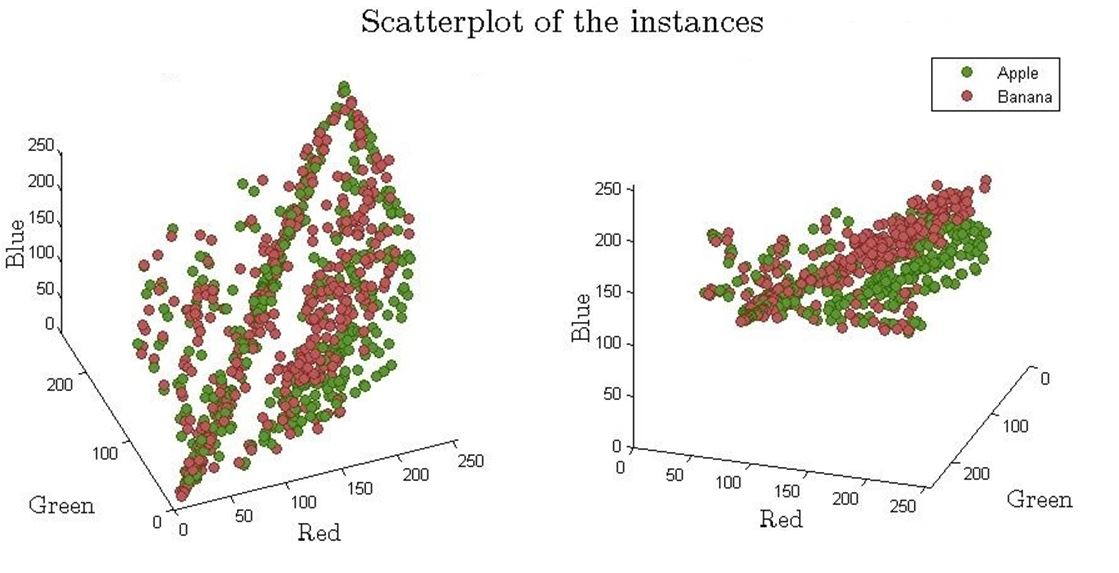
\includegraphics[width = \textwidth]{Images/scatter.png}
		\caption{Decision boundary of decision stump using data from two normal distributions with the identity as covariance matrix and mean $[0,0]^{T}, [0,2]^{T}$ respectively. In the left image, the original data was used whereas in the right image, the second feature was scaled by a factor $3$.}
		\label{fig:scatter}
	\end{figure}
	
	\section*{d.}
	The implementation of the decision stump is tested on the dataset \texttt{optdigitsubset}. If the first 50 objects of each class are used as training data, the accuracy on the remaining test data is $0.98$. Next, the decision stump is trained using a random subset of $50$ examples and tested on the remaining data. This procedure was repeated $50$ times, resulting in a mean accuracy of $0.96$ with standard deviation $0.04$. This result indicates that the data of the two classes are (nearly) separable in at least one of the features. Thus, the high accuracy obtained when using the first 50 objects of each class as training data is not unreasonably high. The code used in this section is shown below.
	\begin{lstlisting}[language=python, frame=l, basicstyle=\ttfamily\scriptsize]
from sklearn.model_selection import ShuffleSplit	

def cross_validate(classifier,X,y,n_splits,train_size):
	splits = ShuffleSplit(n_splits=n_splits, train_size=train_size).split(X)
	scores = []
	for train_indices, test_indices in splits:
		estimator = DecisionStump()
		estimator.fit(X[train_indices,:], y[train_indices])
		scores.append(estimator.score(X[test_indices,:],y[test_indices]))
		return np.array(scores)

def testDecisionStump(X,y):
	mask = np.zeros(len(y), dtype=bool)
	mask[np.concatenate((np.where(y==-1)[0][0:50],np.where(y==1)[0][0:50]))]=True
	stump = DecisionStump()
	stump.fit(X[mask,:],y[mask])
	first = stump.score(X[~mask,:],y[~mask])
	scores = cross_validate(DecisionStump,X,y,n_splits=50, train_size=50)
	print("Using first 50 of both classes as training data:\nscore: {}\n".format(first))
	print("Decision stump accuracy with random subsets:\nmean: {}, std: {}\n".format(scores.mean(),scores.std()))
	\end{lstlisting}
	
	\section*{e.}
	To whether or not the decision stump accepts and handles weights properly, data corresponding to one of the classes are weighted four times heavier. The data was generated as in \textbf{c.} The resulting decision boundaries are shown in figure \ref{weights}. It can be seen that the decision boundary favours the more heavily weighted class, as expected.
	
	\begin{figure}[H]
		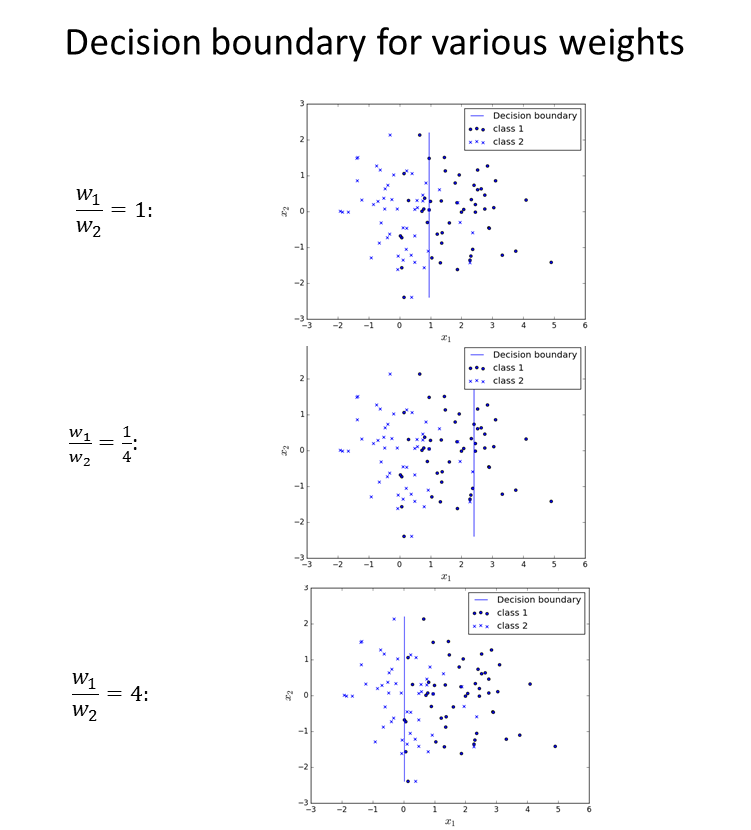
\includegraphics[width = \textwidth]{Images/weights.png}
		\caption{Decision boundary of decision stump using differently weighted data. The data is obtained as in \textbf{c.}}
		\label{weights}
	\end{figure}
	\newpage
	\section*{f.}
	The implementation of the AdaBoost algorithm is shown below.
	
	\begin{lstlisting}[language=python, frame=l, basicstyle=\ttfamily\scriptsize]		
class AdaBoostClassifier():
	def __init__(self, iterations, WeakLearner):
		self.WeakLearner, self.learners, self.weights, self.errors, self.N = WeakLearner, [], [], [], iterations
		self.objectWeights = []
	
	def expectedLabels(self,X):
		weightedPredictions = [self.weights[l]*learner.predict(X) for l,learner in enumerate(self.learners)]
		return np.array(weightedPredictions).sum(axis=0)
	
	def predict(self,X):
		return [1 if e>0 else -1 for e in self.expectedLabels(X)]
	
	def score(self, X, y):
		return sum([1 if fxi==y[i] else 0 for i,fxi in enumerate(self.predict(X))])/y.shape[0] 
	
	def fit(self, X, y):
		objectWeights = lambda: np.exp(-y*self.expectedLabels(X))
		self.learners, self.weights, self.errors, w = ([],[],[], np.ones(X.shape[0]))
		for i in range(0,self.N):
			newLearner = self.WeakLearner()
			newLearner.fit(X,y,w=w)
			error = (1-newLearner.accuracy)
			self.weights.append(0.5*m.log(1/(error+1e-10)-1))
			self.learners.append(newLearner)
			totalError = 1 - self.score(X,y)
			self.errors.append(totalError)
			w = objectWeights()
			if totalError<1e-5:
				break
		self.objectWeights = w 
	\end{lstlisting}
	
	\section*{g.}
	in figures \ref{decision_boundary1} and \ref{decision_boundary2}, the decision boundary of the classifier is shown in color after various number of iterations $N$ and the training data is plotted as a scatter plot. It can be seen that with increasing number of iterations, the prediction of the classifier agrees more and more with the training data, as expected. Furthermore, it can be seen that the more difficult/poorly predicted objects get a higher weight.
	
	\begin{figure}[H]
		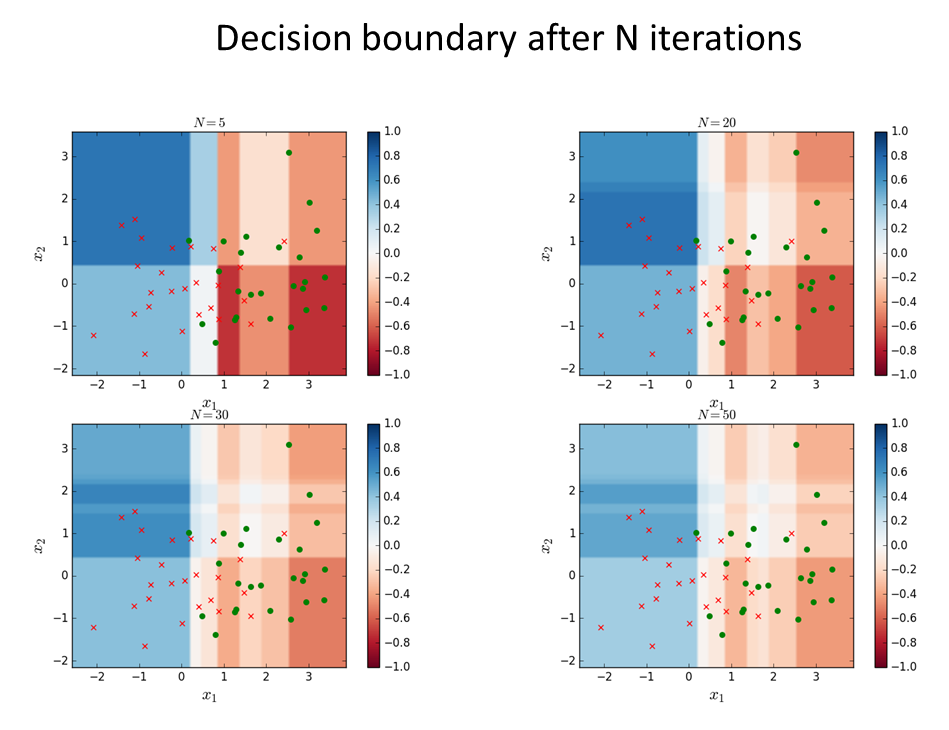
\includegraphics[width = \textwidth]{Images/decision_boundary.png}
		\caption{Decision boundary after $N$ iterations. The training data is shown as a scatter plot and the yellow circles indicate the five objects with the highest weight at the last performed iteration. }
		\label{decision_boundary1}
	\end{figure}

	\begin{figure}[H]
		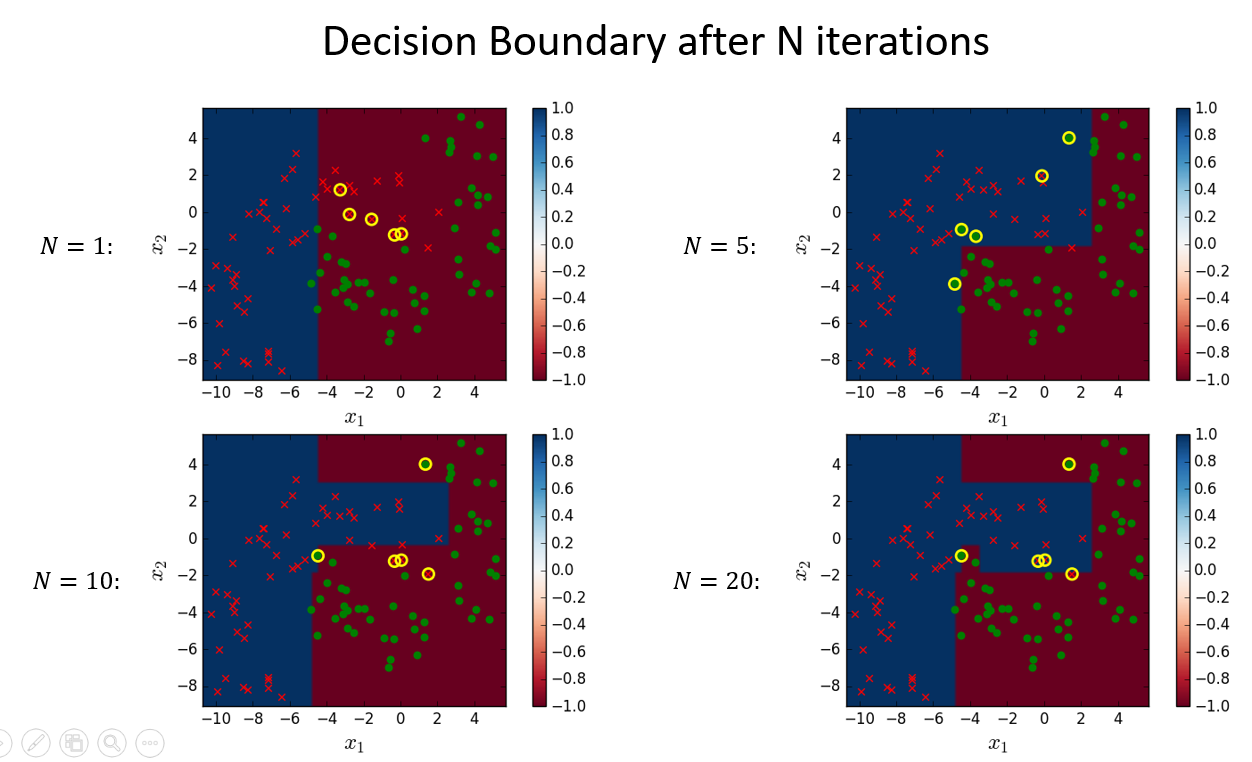
\includegraphics[width = \textwidth]{Images/decision_boundary2.png}
		\caption{Decision boundary after $N$ iterations. The training data is shown as a scatter plot and the yellow circles indicate the five objects with the highest weight at the last performed iteration.}
		\label{decision_boundary2}
	\end{figure}
	
	\section*{h}
	The implementation is tested on the dataset \texttt{optdigitsubset}, using the first 50 object of each class as training data and the rest as test data. The resulting accuracy is plotted for various number of maximum iterations in figure \ref{accuracy}. It can be seen that after just a few iterations, the accuracy remains approximately constant at 0.9864. Comparing this with \textbf{d.}, this result was to be expected, as it was indicated that the data is (nearly) separable.
	
	\begin{figure}[H]
		\begin{center}
			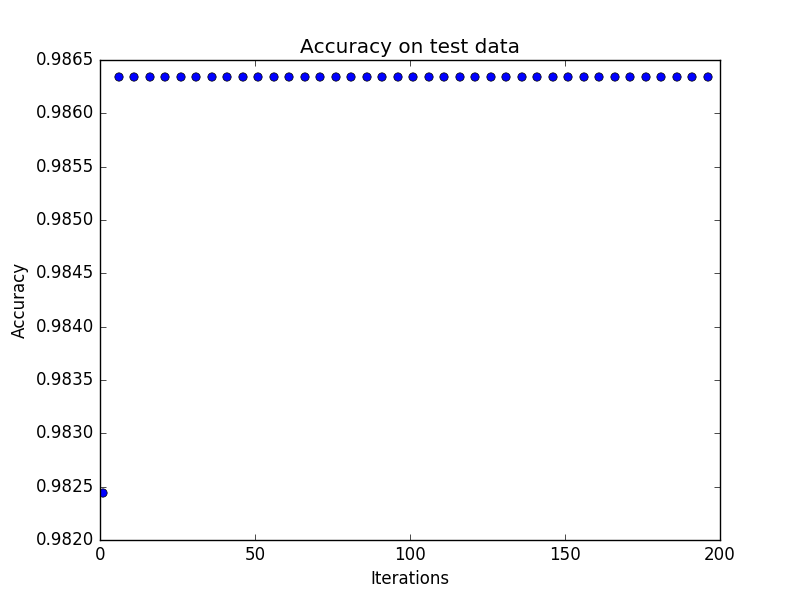
\includegraphics[scale=0.5]{Images/accuracy.png}
			\caption{Accuracy of the AdaBoost classifier on the \texttt{optdigitsubset} dataset for various number of iterations.}
			\label{accuracy}
		\end{center}
	\end{figure}
	\newpage \noindent
	In figure \ref{high_weight}, images that got a high weight during the fitting process are compared to three random images of the two classes. It is clear that the highly weighted images are the more difficult to classify objects, which also explains why they got a higher weight.
	
	\begin{figure}[H]
		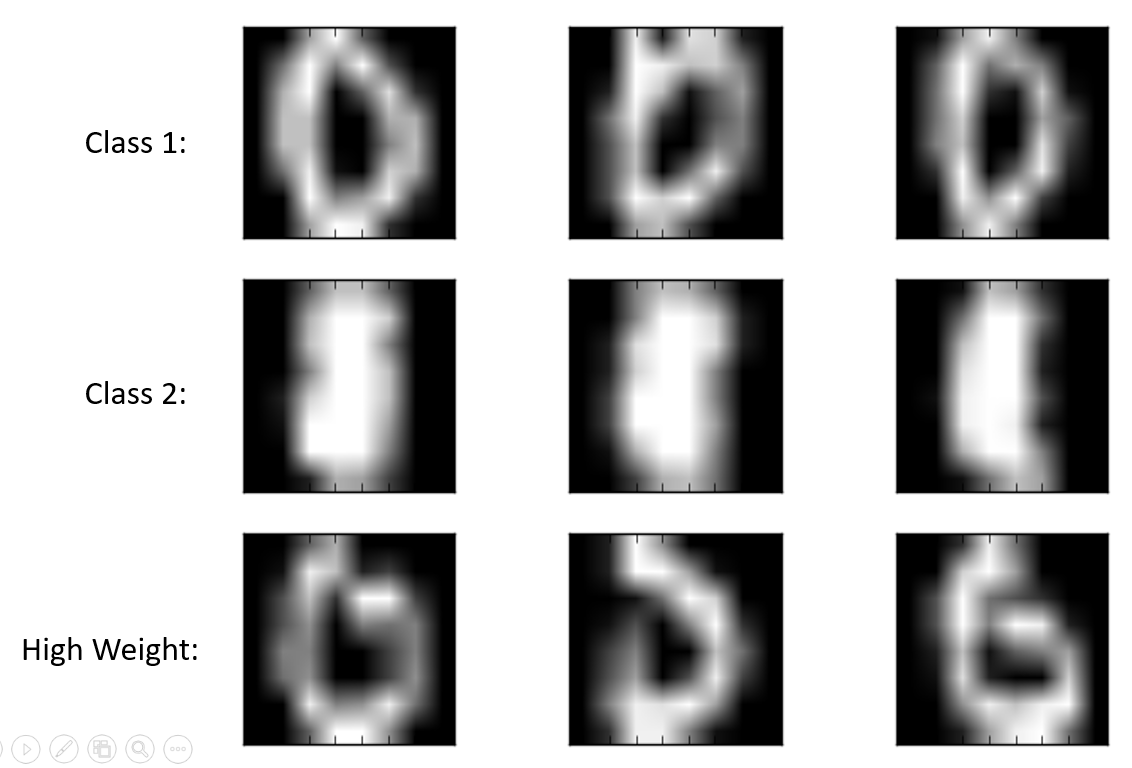
\includegraphics[width = \textwidth]{Images/images1.png}
		\caption{The three images that got the highest weight in the fitting process compared to three images of the two classes.}
		\label{high_weight}
	\end{figure}

\end{document}